% Auto-generated by figures/generate_rqr_theory_figures.R.
% Text-native Figure 2 source for Overleaf/GitHub transport.
% content=0.8; RQR=0.000000; ET=0.140204; SH=0.292760; CF_ET=0.168459; CF_SH=0.505378
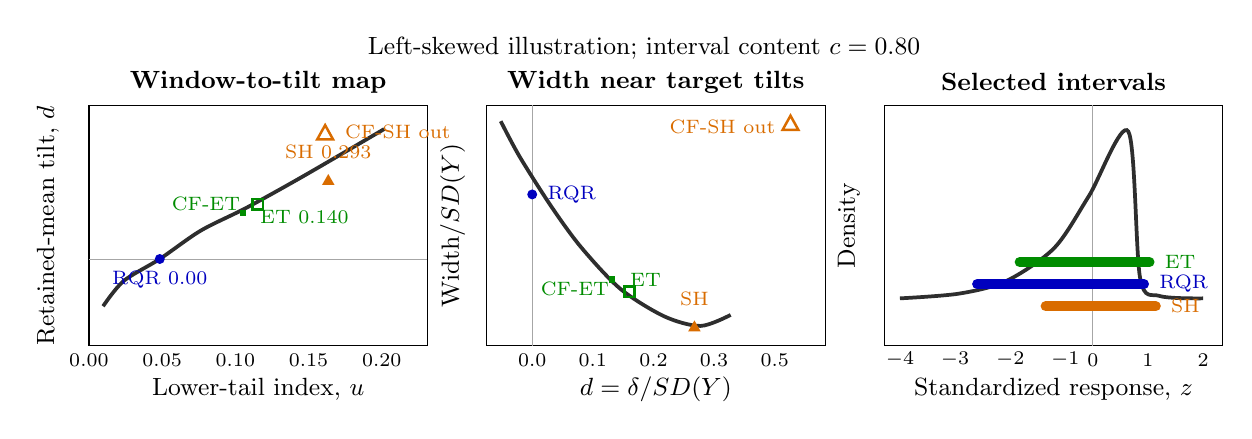
\begin{tikzpicture}[x=1cm,y=1cm,
  axis/.style={draw=black,line width=0.45pt},
  curve/.style={line width=1.35pt,draw=black!82},
  rqr/.style={blue!75!black},
  et/.style={green!55!black},
  sh/.style={orange!85!black},
  cf/.style={line width=0.9pt},
  lab/.style={font=\scriptsize},
  title/.style={font=\bfseries\small},
  tick/.style={font=\scriptsize}]
\node[font=\small] at (7.05,3.78) {Left-skewed illustration; interval content $c=0.80$};

% Panel A: window-to-tilt map.
\begin{scope}[shift={(0,0)}]
\node[title] at (2.15,3.35) {Window-to-tilt map};
\draw[axis] (0,0) rectangle (4.3,3.05);
\draw[black!35,line width=0.35pt] (0,1.10) -- (4.3,1.10);
\draw[curve] plot[smooth] coordinates {(0.18,0.50) (0.44,0.82) (0.90,1.10) (1.42,1.46) (2.00,1.75) (2.72,2.15) (3.75,2.75)};
\fill[rqr] (0.90,1.10) circle (1.8pt);
\node[lab,rqr,below=1pt] at (0.90,1.10) {RQR 0.00};
\fill[et] (1.92,1.64) rectangle ++(0.08,0.08);
\node[lab,et,right=2pt] at (1.98,1.63) {ET 0.140};
\draw[et,cf] (2.08,1.73) rectangle ++(0.13,0.13);
\node[lab,et,left=1pt] at (2.08,1.80) {CF-ET};
\fill[sh] (3.04,2.18) -- ++(-0.08,-0.14) -- ++(0.16,0) -- cycle;
\node[lab,sh,above=2pt] at (3.04,2.18) {SH 0.293};
\draw[sh,cf] (3.00,2.80) -- ++(-0.10,-0.18) -- ++(0.20,0) -- cycle;
\node[lab,sh,right=2pt] at (3.06,2.71) {CF-SH out};
\node[tick] at (0,-0.18) {0.00};
\node[tick] at (0.93,-0.18) {0.05};
\node[tick] at (1.86,-0.18) {0.10};
\node[tick] at (2.79,-0.18) {0.15};
\node[tick] at (3.72,-0.18) {0.20};
\node[font=\small] at (2.15,-0.55) {Lower-tail index, $u$};
\node[font=\small,rotate=90] at (-0.52,1.52) {Retained-mean tilt, $d$};
\end{scope}

% Panel B: width profile.
\begin{scope}[shift={(5.05,0)}]
\node[title] at (2.15,3.35) {Width near target tilts};
\draw[axis] (0,0) rectangle (4.3,3.05);
\draw[black!35,line width=0.35pt] (0.58,0) -- (0.58,3.05);
\draw[curve] plot[smooth] coordinates {(0.18,2.85) (0.42,2.40) (0.82,1.77) (1.20,1.25) (1.70,0.72) (2.26,0.37) (2.72,0.25) (3.10,0.39)};
\fill[rqr] (0.58,1.92) circle (1.8pt);
\node[lab,rqr,right=2pt] at (0.58,1.92) {RQR};
\fill[et] (1.55,0.80) rectangle ++(0.08,0.08);
\node[lab,et,right=2pt] at (1.63,0.84) {ET};
\draw[et,cf] (1.75,0.62) rectangle ++(0.13,0.13);
\node[lab,et,left=2pt] at (1.75,0.72) {CF-ET};
\fill[sh] (2.64,0.32) -- ++(-0.08,-0.14) -- ++(0.16,0) -- cycle;
\node[lab,sh,above=2pt] at (2.64,0.32) {SH};
\draw[sh,cf] (3.86,2.92) -- ++(-0.10,-0.18) -- ++(0.20,0) -- cycle;
\node[lab,sh,left=2pt] at (3.86,2.78) {CF-SH out};
\node[tick] at (0.58,-0.18) {0.0};
\node[tick] at (1.35,-0.18) {0.1};
\node[tick] at (2.12,-0.18) {0.2};
\node[tick] at (2.89,-0.18) {0.3};
\node[tick] at (3.66,-0.18) {0.5};
\node[font=\small] at (2.15,-0.55) {$d=\delta/\operatorname{SD}(Y)$};
\node[font=\small,rotate=90] at (-0.43,1.52) {Width$/\operatorname{SD}(Y)$};
\end{scope}

% Panel C: selected intervals.
\begin{scope}[shift={(10.10,0)}]
\node[title] at (2.15,3.35) {Selected intervals};
\draw[axis] (0,0) rectangle (4.3,3.05);
\draw[black!35,line width=0.35pt] (2.65,0) -- (2.65,3.05);
\draw[curve] plot[smooth] coordinates {(0.20,0.60) (0.95,0.66) (1.55,0.82) (2.16,1.24) (2.60,1.90) (3.10,2.72) (3.25,0.86) (3.50,0.63) (4.05,0.60)};
\draw[et,line width=3.6pt,line cap=round] (1.72,1.06) -- (3.37,1.06);
\node[lab,et,right=2pt] at (3.37,1.06) {ET};
\draw[rqr,line width=3.6pt,line cap=round] (1.18,0.78) -- (3.30,0.78);
\node[lab,rqr,right=2pt] at (3.30,0.78) {RQR};
\draw[sh,line width=3.6pt,line cap=round] (2.05,0.50) -- (3.45,0.50);
\node[lab,sh,right=2pt] at (3.45,0.50) {SH};
\node[tick] at (0.20,-0.18) {$-4$};
\node[tick] at (0.90,-0.18) {$-3$};
\node[tick] at (1.60,-0.18) {$-2$};
\node[tick] at (2.30,-0.18) {$-1$};
\node[tick] at (2.65,-0.18) {$0$};
\node[tick] at (3.35,-0.18) {$1$};
\node[tick] at (4.05,-0.18) {$2$};
\node[font=\small] at (2.15,-0.55) {Standardized response, $z$};
\node[font=\small,rotate=90] at (-0.45,1.52) {Density};
\end{scope}
\end{tikzpicture}
